\documentclass[12pt,a4paper]{article}

\usepackage[pdftex,
            pdfauthor={Hannes Braun},
            pdftitle={Jhin3 user manual},
            pdfsubject={Jhin3}]{hyperref}
\usepackage{graphicx}
\usepackage{fancyhdr}
\usepackage{listings}
\usepackage{xcolor}

\lstdefinelanguage{json}{
    basicstyle=\normalfont\ttfamily,    
    showstringspaces=false,
    breaklines=true,
    backgroundcolor=\color{lightgray}
}

\renewcommand{\familydefault}{\sfdefault}

\begin{document}

\pagenumbering{arabic}

\pagestyle{fancy}
\lhead{Jhin3 user manual}
\rhead{Page \thepage}
\cfoot{}

\thispagestyle{empty}
\begin{center}
\begin{Huge}
\textbf{Jhin3}
\end{Huge}

\begin{Large}
\vspace{0.4cm}
\textbf{Console soundboard}
\end{Large}

\begin{large}
\vspace{0.1cm}
User manual

\vspace{1cm}

Version 2020.0.0

\vspace{0.7cm}

Copyright \textcopyright{} 2020 Hannes Braun

\href{https://github.com/hannesbraun/jhin3}{https://github.com/hannesbraun/jhin3}
\end{large}

\vspace{2.4cm}
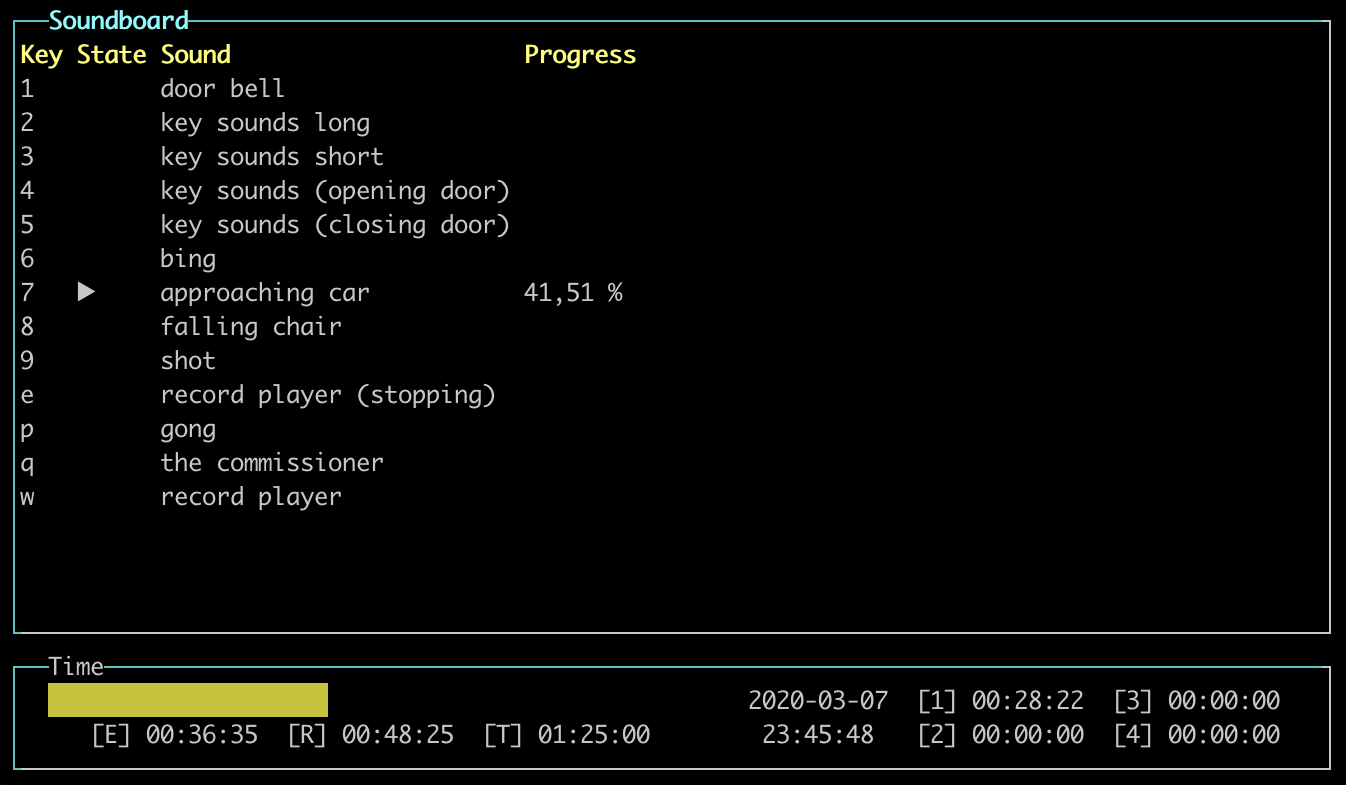
\includegraphics[scale=0.6]{../preview.png}

\end{center}
\newpage

\tableofcontents
\newpage

\section{Introduction}

Jhin3 is a console soundboard with some additional timer and stopwatch functionality.

The main features are:
\begin{itemize}
\item Soundboard with 3 different sound types (normal, loop and one shot)
\item Configurable through a json file
\item Timer
\item 4 stopwatches
\item Different themes to choose from
\end{itemize}

This manual is still not complete yet. I will extend it together with further releases in the future. However, it should contain the necessary information to run Jhin3.

\newpage

\section{Installation}

So you decided to give Jhin3 a try? Great!
To run Jhin3, you need to have Java (version 8 or higher) installed. This makes Jhin3 compatible with all the major operating systems such as Linux, macOS and Windows. Jhin3 itself is nothing more than a jar file. This means that you can either install Jhin3 to a system directory or just put the jar file somewhere you like in your user directory. Decide for yourself what suits to your needs.

\subsection{Getting the jar file}

You can either download a pre-built version of Jhin3 from the GitHub releases page or you can build Jhin3 yourself.

\subsubsection{Downloading a pre-built version (recommended)}

Go to the GitHub releases page of Jhin3 (\href{https://github.com/hannesbraun/jhin3/releases}{or click here}). Select the latest version and download the associated zip file. It is called something like ``jhin3-2020.0.0.zip''.
Unpack the file and you will find the jar file inside.

\subsubsection{Building from source}

To build Jhin3 from source, make sure you have a JDK (version 8 or higher) installed as well as Maven.

Clone the Jhin3 repository to your computer and navigate to its root directory. Now, just run this command:
\begin{lstlisting}[language=bash]
mvn package
\end{lstlisting}

Inside of the target directory, you should find a file called ``jhin3-\{version\}-jar-with-dependencies.jar''.

\subsection{Optional: installing Jhin3}

Right now, you need to type
\begin{lstlisting}[language=bash]
java -jar /path/to/jhin3.jar
\end{lstlisting}
every time you want to run Jhin3. To simplify this, you can install Jhin3 to a system directory and execute it just by typing
\begin{lstlisting}[language=bash]
jhin3
\end{lstlisting}

\subsubsection{Linux/macOS}

In the /opt directory of your system, create a new directory called ``jhin3''. Rename the Jhin3 jar file to ``jhin3.jar'' and move it into this new directory.
Next, create a file called ``jhin3'' inside of ``/usr/local/bin''. This serves as a wrapper for the actual jar file.
Copy the following code inside that file:

\begin{lstlisting}[language=bash]
#!/bin/sh

java -jar /opt/jhin3/jhin3.jar "$@"
\end{lstlisting}

You should now be able to run Jhin3 anywhere by typing:
\begin{lstlisting}[language=bash]
jhin3
\end{lstlisting}

To update Jhin3, replace ``/opt/jhin3/jhin3.jar'' with the new jar file.

\section{The configuration file}

To use Jhin3, you need to have a configuration file in the JSON format. If you are unfamiliar with JSON, don't worry. There is a lot of documentation on the internet about JSON and you can also check out the sample configuration in the repository of this project (\href{https://github.com/hannesbraun/jhin3/blob/master/sample_conf.json}{click here}).

Every sound entry should look something like this:
The first property called ``soundboard\_name'' is unused at the moment. You can add it to your configuration file and provide a name for this soundboard, it doesn't matter right now.
With ``resource\_folder'', you provide the base directory for your sounds. This should minimize the amount of typing for the path of the sound files.

\textbf{Important note:} only wav and aiff files are supported at the moment. (You can convert other files to wav or aiff by using for example \href{https://ffmpeg.org}{ffmpeg}.)

The object ``sounds'' contains all your desired sounds. A sound entry looks like this:
\begin{lstlisting}[language=json]
"1": {
        "filename": "awesome_sound.wav",
        "description": "My awesome sound",
        "active": true,
        "type": "normal",
        "terminate": true,
        "fadein": 4.2,
        "fadeout": 0.0,
        "volume": 0.0,
        "pan": 0.0
}
\end{lstlisting}

\begin{itemize}
\item ``filename'': the path to your sound file.
\item ``description'': the description displayed inside of Jhin3
\item ``active'': if set to true, the sound will show up as expected. By setting this to false, the sound will be ignored by Jhin3. This is useful if you have a sound but you don't need it yet. At any time, you can just set this flag to true and your sound will be available.
\item ``type'': the type of the sound. Three types are available: ``normal'', ``loop'' and ``oneshot''.
	\begin{itemize}
	\item ``normal'': pressing the associated key will start and stop the sound with the provided fadein and fadeout. If the sound has finished playing because, nothing else happens and the fadeout won't be applied.
	\item ``loop'': works like ``normal'' but if the sound has finished playing it will start from the beginning again
	\item ``oneshot'': ignores ``fadein''. If the sound is playing and the associated key is pressed, the sound will play again starting from the beginning.
	\end{itemize}
\item ``terminate'': only used for the type ``oneshot''. Determines if the old sound will stop playing when starting a new sound. If not, multiple instances of the sound will play at the same time.
\item ``fadein'': fade-in time in seconds
\item ``fadeout'': fade-out time in seconds
\item ``volume'': gain in dB applied to the sound. 0.0 leaves the volume untouched. Values from -79.9 to 6.0 are possible.
\item ``pan'': panning of the sound. Values from -1.0 (left) to 1.0 (right) are possible.
\end{itemize}

\newpage

\section{Using Jhin3}

\textbf{Important note:} For windows, use javaw instead of java.

\subsection{Command line options}

The following command line options are available:
\begin{itemize}
\item ``-b [buffer size]'': audio buffer size in ms
\item ``-c [path]'': path to the configuration file
\item ``-t [theme]'': theme to use (currently available: ``2019'', ``2020'', ``bsod'' and ``frost-archer'')
\item ``--version'': only prints the header including the version number (and exits afterwards)
\end{itemize}

\subsection{General usage}

To switch between the soundboard and the time window press ``ctrl-F''.

In the soundboard window, you can press any of the mapped keys (defined inside of the given configuration file). This will trigger the sound depending on its type.
The column ``state'' shows if the sound is fading in, playing or fading out. The progress column shows the playing progress of the last started instance of the sound.

In the time window, you can start and stop the timer by pressing ``S''. To reset the timer, press ``C''.
Changing the timer duration is possible by pressing ``X''. The maximum length is 99 hours, 59 minutes and 59 seconds. The input has to be of the form HH:mm:ss.

The four stopwatches can be started and stopped by pressing ``1'', ``2'', ``3'' or ``4''. To reset them, press ``Q'', ``W'', ``E'' and ``R'' respectively.

To exit Jhin3 press the esc-key.

\end{document}